\documentclass[a4paper]{article}
\usepackage{import}
\usepackage{graphicx}
\usepackage{float}
\usepackage{pgfplots}
\usepackage{listings}
\usepackage{enumitem}
\usepackage{textcomp}
\usepackage{tikz}
\usetikzlibrary{decorations.pathreplacing} % for angle arc
\usetikzlibrary{angles, quotes, calc, positioning, trees} % for drawing angles
\pgfplotsset{compat=1.18,width=10cm}
\usepackage{tikz-cd}
\usepackage{booktabs}
\usepackage{cancel}
\usepackage{amsmath}
\usepackage{minted}
\usepackage{csquotes}
\usepackage{gensymb}
\usepackage{forest}
\usepackage{amsthm}
\usepackage{amssymb}
\usepackage{fontawesome} 
\usepackage{varwidth}
\usepackage{pgfplots}
\usepackage{lipsum}
\usepackage{mdframed} 
\usepackage{color}   
\usepackage{hyperref}
\newmdtheoremenv{theo}{Theorem}
\usepackage{mathtools}
\DeclarePairedDelimiter\ceil{\lceil}{\rceil}
\DeclarePairedDelimiter\floor{\lfloor}{\rfloor}

\hypersetup{
    colorlinks=true, %set true if you want colored links
    linktoc=all,     %set to all if you want both sections and subsections linked
    linkcolor=black,  %choose some color if you want links to stand out
}

% Define theorem styles
\newtheorem{theorem}{Theorem}[section]    % Theorems numbered within sections
\newtheorem{lemma}[theorem]{Lemma}        % Lemmas use the same counter as theorems
\newtheorem{corollary}[theorem]{Corollary} % Corollaries use the same counter as theorems
\newtheorem{proposition}[theorem]{Proposition} % Proposition uses the same counter
\newtheorem{property}[theorem]{Property}
\theoremstyle{definition}
\newtheorem{definition}[theorem]{Definition} % Now uses the same counter as theorems


% Remark-style theorem
\theoremstyle{remark}
\newtheorem{remark}[theorem]{Remark}

% Boxed environment for theorems
\newmdenv[
  linewidth=0.8pt,
  roundcorner=5pt,
  linecolor=black,
  backgroundcolor=white!5,
  skipabove=\baselineskip,
  skipbelow=\baselineskip,
  innerleftmargin=10pt,
  innerrightmargin=10pt,
  innertopmargin=5pt,
  innerbottommargin=5pt
]{thmbox}

% Custom proof environment (also boxed)
\renewenvironment{proof}[1][Proof]{%
  \begin{mdframed}[linewidth=0.8pt, roundcorner=5pt, linecolor=black, skipabove=\baselineskip, skipbelow=\baselineskip, innertopmargin=5pt, innerbottommargin=5pt]%
  \noindent\textbf{#1. }%
}{%
  \end{mdframed}%
}

% Redefine theorem environments to use thmbox
\let\oldtheorem\theorem
\renewenvironment{theorem}{\begin{thmbox}\begin{oldtheorem}}{\end{oldtheorem}\end{thmbox}}

\let\oldlemma\lemma
\renewenvironment{lemma}{\begin{thmbox}\begin{oldlemma}}{\end{oldlemma}\end{thmbox}}

\let\oldcorollary\corollary
\renewenvironment{corollary}{\begin{thmbox}\begin{oldcorollary}}{\end{oldcorollary}\end{thmbox}}

\let\oldproposition\proposition
\renewenvironment{proposition}{\begin{thmbox}\begin{oldproposition}}{\end{oldproposition}\end{thmbox}}

\let\oldproperty\property
  \renewenvironment{property}{\begin{oldproperty}}{\end{oldproperty}}


% Reference shortcuts
\newcommand{\thmref}[1]{Theorem~\ref{#1}}
\newcommand{\lemref}[1]{Lemma~\ref{#1}}
\newcommand{\corref}[1]{Corollary~\ref{#1}}
\newcommand{\propref}[1]{Property~\ref{#1}} 

% To customize QED symbol
\renewcommand{\qedsymbol}{$\blacksquare$}

\usetikzlibrary{decorations.pathreplacing} % for angle arc
\usetikzlibrary{angles, quotes, calc} % for drawing angles

\usepackage{color}   %May be necessary if you want to color links
\usepackage{hyperref}
\hypersetup{
    colorlinks=true, %set true if you want colored links
    linktoc=all,     %set to all if you want both sections and subsections linked
    linkcolor=black,  %choose some color if you want links to stand out
}

\usepackage{xcolor}
\usepackage[most]{tcolorbox}


% Define a custom tcolorbox environment for examples
\newtcolorbox{examplebox}[2][]{
  colback=blue!5!white,
  colframe=blue!30!black,
  title=#2,
  boxrule=0mm,
  fonttitle=\bfseries,
  width=\textwidth,
  breakable,
  #1
}

\newtcolorbox{definizione}[2] {
  colback=green!5!white,
  colframe=green!30!black,
  title=#2,
  boxrule=0mm,
  fonttitle=\bfseries,
  width=\textwidth,
  breakable,
  #1
}

\definecolor{codegreen}{rgb}{0,0.6,0}
\definecolor{codegray}{rgb}{0.5,0.5,0.5}
\definecolor{codepurple}{rgb}{0.58,0,0.82}
\definecolor{backcolour}{rgb}{0.95,0.95,0.92}

\lstdefinestyle{mystyle}{
    backgroundcolor=\color{backcolour},   
    commentstyle=\color{codegreen},
    keywordstyle=\color{magenta},
    numberstyle=\tiny\color{codegray},
    stringstyle=\color{codepurple},
    basicstyle=\ttfamily\footnotesize,
    breakatwhitespace=false,         
    breaklines=true,                 
    captionpos=b,                    
    keepspaces=true,                 
    numbers=left,                    
    numbersep=5pt,                  
    showspaces=false,                
    showstringspaces=false,
    showtabs=false,                  
    tabsize=2
}

\lstset{style=mystyle}

\makeatletter
\renewcommand*\env@matrix[1][*\c@MaxMatrixCols c]{%
  \hskip -\arraycolsep
  \let\@ifnextchar\new@ifnextchar
  \array{#1}}
\makeatother

\title{Operating Systems - Paper on Input/Output Devices}
\author{SETU - South East Technological University\\Imbriani Paolo - W20114452\\Professor Micheal McMahon}

\begin{document}

\begin{figure}
    \centering
    
\includegraphics[width=0.6\textwidth]{SETU.png}
    \label{fig:centered-image}
\end{figure}

\maketitle 

\begin{abstract}
    Input/Output (I/O) systems are essential for how a computer’s processor communicates with 
    external devices. This dissertation explores the structure, design, and performance of I/O systems. 
    It covers both hardware components, like device controllers, interfaces, and direct memory access, 
    as well as software mechanisms, such as device drivers, I/O scheduling, and caching. Lastly, 
    it discusses new advancements, including high-speed connections, challenges in virtualization,
    and the use of AI in managing I/O, showing how these systems continue to evolve in modern computing.
\end{abstract}


\pagebreak

\tableofcontents

\pagebreak

\section*{Introduction}

Input/Output systems, simply put, enable computers to interact with its environment.
They connect the central processing unit (CPU) with various peripheral devices—ranging from 
keyboards and displays, to storage systems and network interfaces. As modern computing demands 
increased speed, efficiency, and reliability, the design and management of I/O systems have become 
critically important. This paper examines the fundamental components of I/O systems and their history, their role 
within operating systems, and the impact of emerging technologies on future developments.

\begin{figure}[H]
    \centering
    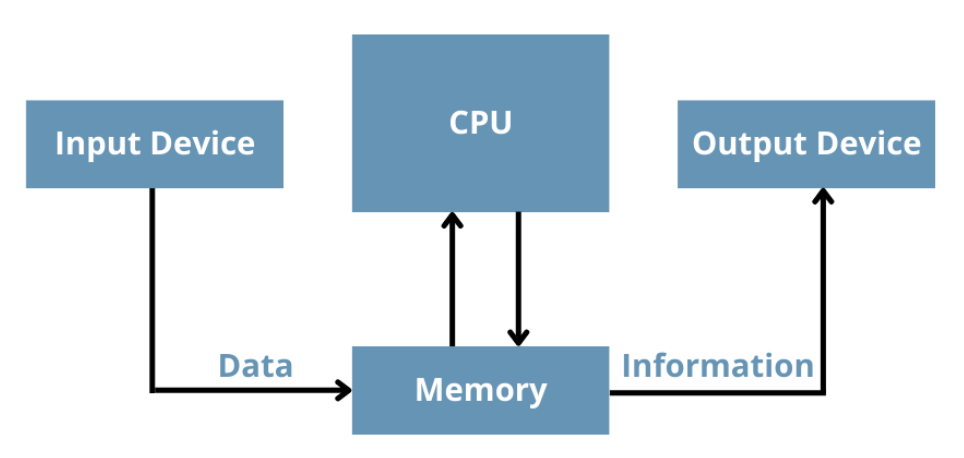
\includegraphics[width=0.6\textwidth]{IO.png}
    \caption{Flow of data between inputs/outputs, memory and processing units.}
\end{figure}

For instance: a user wants to type a document on a computer.
In this scenario, the keyboard would be the input device. 
By pressing letter, number, and symbol keys, a user can submit data and
instructions to the computer. Each key is transformed into a \textit{binary number} that the
CPU can \textit{interpret and recognize}. This is stored in the system’s memory and transferred 
to the CPU to perform its calculations to provide an output result. 
Then, this is information is displayed in the output device, such as a monitor.



\section{Overview of I/O Systems}

I/O systems connects both hardware and software elements that coordinate data 
exchange between the CPU and peripheral devices. Key functions include:

\begin{itemize}
    \item \textbf{Data Transfer}: Moving data to and from peripherals.
    \item \textbf{Control}: Managing device operations and status.
    \item \textbf{Error Handling}: Detecting and recovering from faults.
\end{itemize}
Efficient I/O systems must balance competing requirements such as throughput, latency, 
and resource utilization to ensure seamless operation [1].


\section{I/O Hardware Components}

The hardware side of I/O systems involves several critical components:

\begin{itemize}
    \item \textbf{Device Controllers}: Interface between the CPU and peripheral devices.
    \item \textbf{Interfaces}: Connect controllers to devices via buses or networks.
    \item \textbf{Direct Memory Access (DMA)}: Enables devices to access memory without CPU intervention.
\end{itemize}
A general-purpose computer system consists of CPUs and multiple device
controllers that are connected through a \textit{common bus}.

\begin{figure}[H]
    \centering
    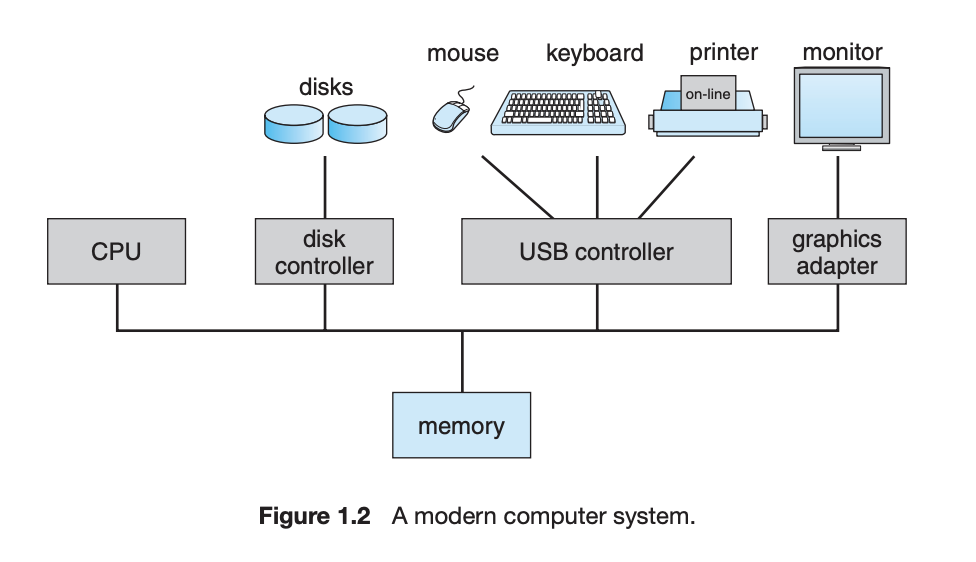
\includegraphics[width=1\textwidth]{Amod.png}
\end{figure}

\subsection{Device Controllers}

Device controllers serve as a bridge between the processing unit and peripheral devices. They interpret the commands issued by 
the operating system and manage the specifics of data transfer. Each device controller
is in charge of a specific type of device. Depending on the controller, more
than one device may be attached.  A device controller maintains some local buffer storage and a set of special-purpose
registers. The device controller is responsible for moving the data between
the peripheral devices that it controls and its local buffer storage. Typically,
operating systems have a device driver for each device controller. This device
driver understands the device controller and provides the rest of the operating
system with a uniform interface to the device.
\\
\vspace{1em}

\noindent
Let's say we want to start an I/O operation. What does the process look like?

\begin{enumerate}
    \item The device driver loads the appropriate registers
    within the device controller.
    \item The device controller, in turn, examines the
    contents of these registers to determine what action to take (such as “read
    a character from the keyboard”).
    \item The controller starts the transfer of data from
    the device to its local buffer. 
    \item Once the transfer of data is complete, the device
    controller informs the device driver via an interrupt that it has finished its
    operation. s
    \item The device driver then returns control to the operating system,
    possibly returning the data or a pointer to the data if the operation was a read.
    For other operations, the device driver returns status information. [1]
\end{enumerate}

\subsection{Interfaces and Buses}

Communication between the CPU and peripherals is facilitated by buses and interfaces. Here some examples:

\begin{itemize}
    \item Peripheral Component Interconnect Express (PCIe): High-speed interface for connecting devices to the CPU.
    \item Universal Serial Bus (USB): Widely used interface for connecting peripherals to computers.
    \item Serial ATA (SATA): Interface for connecting storage devices to the motherboard.
\end{itemize}
These interfaces are widely spread in the world and now standardized in the world of communication protocols and ensure that data is transferred efficienctly and reliably.

\subsection{Direct Memory Access (DMA)}

When CPU need to fetch an instruction or data from memory, it always controls the status of the device and that could be done using \textbf{interrupts} that is a hardware signals 
that interrupts the normal flow of execution only when the device is ready. But to
 transfer large amounts of data from an input/output device to memory, it is
not advisable to use interrupts because it would be a waste of resources. DMA is used, which 
is a device that allows data to be transferred from memory to the input/output device without passing 
through the CPU. [1] [2]


\begin{figure}[H]
    \centering
    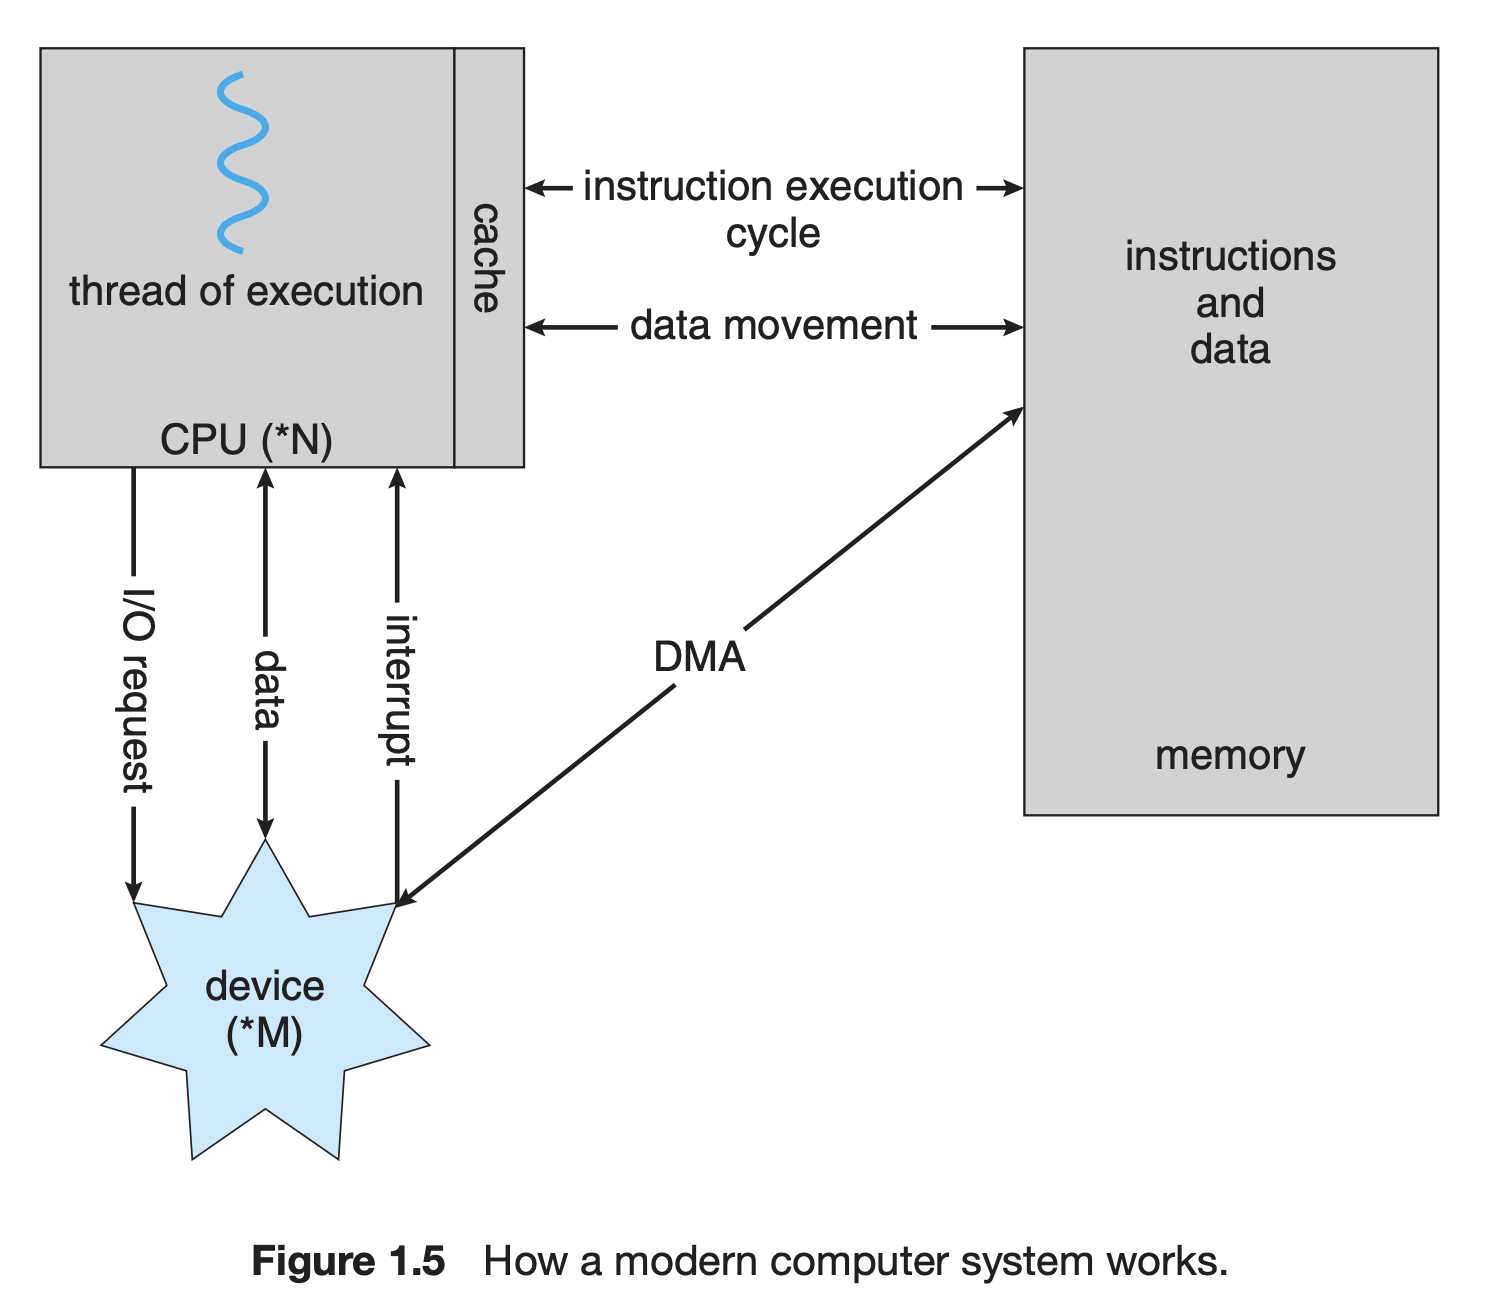
\includegraphics[width=0.6\textwidth]{DMA.png}
\end{figure}

\section{I/O Software and Operating System Support}

The software layer of I/O systems is very important since it has to manage hardware resources effectively and efficienctly.

\subsection{Device Drivers}

Device drivers are specialized software modules that serve as the crucial bridge between the operating system and hardware peripherals. They translate high-level operating system commands into the low-level instructions required by specific hardware devices, ensuring that each device operates according to its unique protocol. Modern operating systems leverage modular driver architectures, allowing drivers to be dynamically loaded as kernel modules. This means that when a new peripheral—such as a USB device or a PCIe card—is connected, the operating system can automatically detect it, determine the appropriate driver, and load that driver without needing a system reboot. [1]

The development and maintenance of device drivers require meticulous attention to performance, security, and system stability. Since drivers operate in kernel space, any malfunction or coding error can compromise the entire system, potentially leading to crashes or security vulnerabilities. As a result, developers adhere to rigorous coding standards and thorough testing procedures. For example, the Linux kernel emphasizes the use of abstraction layers to separate hardware-specific logic from core system functions, while Windows employs frameworks like the Windows Driver Model (WDM) and Windows Driver Frameworks (WDF) [5] to streamline driver development and enhance reliability.

Furthermore, virtualizing I/O poses an increasingly complex challenge as the number and variety of peripheral devices continue to expand. Virtual I/O drivers must not only support a broad range of device-specific idiosyncrasies but also present a consistent interface to the operating system. This is particularly important in virtualized environments, such as cloud platforms, where multiple virtual machines may share a single set of physical hardware resources. The implementation of hot-plug mechanisms and dynamic driver installation has advanced considerably, enabling seamless integration of new devices and reducing the need for manual intervention. [4]

\subsection{I/O Scheduling}

I/O scheduling is a fundamental process in operating system design, aimed at optimizing the order in which input/output requests are processed. Its primary objectives are to minimize wait times, reduce overall latency, and evenly distribute the workload across multiple devices. Efficient I/O scheduling is especially critical in environments with high levels of concurrent I/O operations, such as data centers, multimedia systems, and database servers.

Operating systems implement a variety of algorithms to manage I/O scheduling. The simplest method, First-Come, First-Served (FCFS), processes requests in the order of their arrival. However, in systems such as disk drives—where the physical movement of the disk head is involved—this approach can lead to significant inefficiencies. More advanced scheduling algorithms have been developed to address these shortcomings. For instance, Shortest Seek Time First (SSTF) minimizes the movement of the disk arm by prioritizing requests closest to the current head position. Additionally, algorithms like SCAN (the elevator algorithm) and its variant C-SCAN further optimize disk access by systematically moving the disk head in one direction, servicing all requests along the way before reversing direction.

\begin{examplebox}{Example} Imagine a disk head currently positioned near the middle of a disk. Three applications submit read requests:

\begin{itemize}
    \item Application A requests data from a block near the outer edge,
    \item Application B requests data from a block adjacent to the current head position, and
    \item Application C requests data from a block near the inner edge.
\end{itemize}
If these requests were processed in the order they arrived, the disk head would have to
 traverse long distances between requests, increasing the average latency. However, by 
 reordering the requests to first service Application B (the nearest request), followed by 
 Application C and then Application A, the total movement of the disk head is minimized, 
 leading to quicker response times. 
\end{examplebox}

Modern operating systems manage I/O scheduling by maintaining separate queues for each device. When an application issues a blocking I/O call, the request is added to the corresponding device’s queue [1]. The I/O scheduler then rearranges the queue based on multiple factors, such as the physical location of the data, the priority of the request, and the need to balance load among competing processes. For example, Linux offers multiple I/O scheduling policies, including the Completely Fair Queuing (CFQ) scheduler [6], which aims to balance disk access across processes, and deadline-based schedulers that prioritize time-sensitive operations. These schedulers are designed to ensure that no single application monopolizes disk resources while still meeting the performance requirements of delay-critical processes, such as those involved in virtual memory management.

\subsection{Caching}

Scheduling I/O operations is one way in which the I/O subsystem improves
the efficiency of the computer. Another way is by using storage space in main
memory or on disk via buffering, caching, and spooling. [1]
In addition to reordering requests, modern I/O scheduling techniques 
integrate caching mechanisms to further boost performance. Frequently accessed data
 is stored in faster memory caches, reducing the number of direct physical I/O operations 
 and thereby minimizing latency. The combination of sophisticated scheduling algorithms with 
 efficient caching strategies is essential for managing high I/O demands in today's complex computing 
 environments. [3]
 \\
    \vspace{1em}

    \noindent
    \textbf{What is a cache?} The cache is a small, fast memory that is inserted between the CPU and the main memory. It stores copies of data that are frequently accessed by the CPU, reducing the time required to fetch data from the main memory.
     Caches are organized into multiple levels, with each level offering progressively faster access times and smaller storage capacities. The use of caches is a fundamental technique for improving system performance, 
     as it minimizes the latency associated with fetching data from slower memory devices. [1]

\subsection{Buffering}

A \textbf{buffer} is a memory area that stores data being transferred between
two devices or between a device and an application. The importance of adding a buffer can be separated in three reasons:
\begin{itemize}
    \item To cope with a speed mismatch between the producer and
    consumer of a data stream
    \item To provide adaptations for devices that
    have different data-transfer sizes
    \item To support copy semantics for application I/O
\end{itemize}
Let's go thorugh each of these reasons briefly:
\begin{itemize}
    \item \textbf{Speed Mismatch}: Suppose, for example, that a file is being sent
    by a modem and it has to be stored into the hard disk. The modem is about a thousand
    times slower than the hard disk. So a buffer is created in main memory to
    accumulate the bytes received from the modem. When an entire buffer of data
    has arrived, the buffer can be written to disk in a \textit{single operation}. Since the
    disk write is not instantaneous and the modem still needs a place to store
    additional incoming data, two buffers are used. After the modem fills the first
    buffer, the disk write is requested. The modem then starts to fill the second
    buffer while the first buffer is written to disk. By the time the modem has filled
    the second buffer, the disk write from the first one should have completed,
    so the modem can switch back to the first buffer while the disk writes the
    second one. This \textbf{double buffering} decouples the producer of data from the
    consumer, thus relaxing timing requirements between them. The need for this
    decoupling is due to the enormous differences
    in device speeds for typical computer hardware. [1]
    \item \textbf{Different Data-transfer sizes}: These type of disparities are common in
    computer networking, where buffers are used widely for fragmentation and
    reassembly of messages. [1]
    \item \textbf{Copy Semantics}: A simple way in which the operating system can
    guarantee copy semantics is for the write() system call to copy the application
    data into a kernel buffer before returning control to the application. The disk
    write is performed from the kernel buffer, so that subsequent changes to the
    application buffer have no effect. Copying of data between kernel buffers and
    application data space is common in operating systems, despite the overhead
    that this operation introduces, because of the clean semantics. [1]
\end{itemize}

\subsection{Performance considerations}

The performance of I/O systems is measured by parameters such as throughput, latency, and energy efficiency.

\begin{itemize}
    \item Throughput refers to the volume of data transferred per unit of time.
    \item Latency is the delay before the commencement of data transfer.
\end{itemize}
Optimizing these parameters ensure that I/O devices meet the right performance requirements.


\subsection{Concurrency and Parallelism and Energy Efficiency}

As systems grow more complex, the ability to handle multiple I/O operations
 concurrently becomes very important. Techniques such as multithreading and 
 parallel processing allow systems to manage simultaneous transfers effectively.
 In portable and data-center environments alike, energy efficiency is a significant concern.
  Nowadays, I/O systems incorporate dynamic power management techniques to minimize energy 
  consumption without compromising performance [2].

\section{Future Directions with I/O Systems}

I/O systems are evolving rapidly to meet the demands of modern computing, trying to add accessisbility and security to the system.

\subsection{High-speed Interfaces}

New interface standards, such as Non-Volatile Memory Express (NVMe),
offer dramatic improvements in data transfer rates, particularly for solid-state storage devices.
These developments enable faster access to data and lower latency, which is critical for applications 
requiring rapid data processing. This interface is optimized for all storage solutions, attached using a variety
of transports including PCI Express®, Ethernet, InfiniBandTM, and Fibre Channel. [7]

\subsection{Virtualization and Cloud Computing}

Virtualization introduces additional layers of abstraction that complicate I/O management. 
In \textbf{cloud computing} environments, ensuring efficient and secure I/O across virtual machines is a 
persistent challenge. Advanced resource allocation and isolation techniques are being developed to
 address these issues.

 \subsection{AI Integration}

 Artificial Intelligence (AI) and machine learning are beginning to play roles in optimizing I/O 
 operations. Predictive algorithms can anticipate data transfer patterns, dynamically adjusting
scheduling policies to enhance performance and reduce bottlenecks [8].

\subsection{Challenges of task allocation in dynamic heterogeneous distributed systems}

\textbf{Dynamic heterogeneous systems} consist of multiple processors with varying capabilities, and both the tasks and available resources change over time. 
Because this variability makes it impossible to know task and resource information in advance, estimations must be made in real time.
To address these challenges, researchers have developed four scheduling algorithms that balance different objectives, such as:

\begin{itemize}
    \item Minimizing the total time required to complete all tasks (makespan)
    \item Distributing the workload evenly among processors
\end{itemize}
These algorithms were tested on a real-world distributed system containing up to 90 processors, using tasks
 from diverse fields like cryptography, bioinformatics, and biomedical engineering.
The findings suggest that \textbf{accounting for estimation errors} when assigning tasks leads to more \textbf{efficient scheduling} than ignoring these errors. Additionally, a simple \textbf{heuristic} approach (when combined 
with estimation error) can sometimes perform nearly as well as more complex,
 well-established evolutionary algorithms. [9]


\begin{thebibliography}{9}
    \bibitem{texbook}
    Silberschatz A, Galvin PG, Gagne G. Operating System Concepts. 9th ed. Wiley; 2013.
    \bibitem{texbook}
    Hennessy J, Patterson D. Computer Architecture: A Quantitative Approach. 5th ed. Morgan Kaufmann; 2011.
    \bibitem{citekey}
    XDA Forums. Information about I/O Schedulers [Internet]. XDA Forums; 2012 Mar. Available from: https://xdaforums.com/t/information-about-i-o-schedulers.1558153/
    \bibitem{citekey}
    VMware Security Blog. Hunting Vulnerable Kernel Drivers [Internet]. 
    VMware; 2023 Oct. Available from: 
    https://blogs.vmware.com/security/2023/10/hunting-vulnerable-kernel-drivers.html
    \bibitem{citekey}
    Microsoft Learn. Driver security checklist - Windows drivers [Internet]. Microsoft; 2025 Feb. Available from: https://learn.microsoft.com/en-us/windows-hardware/drivers/driversecurity/driver-security-checklist
    \bibitem{citekey}
    Unix Stack Exchange. Which Scheduling algorithm is used in Linux? [Internet]. Unix Stack Exchange; 2011 Oct. Available from: https://unix.stackexchange.com/questions/20135/which-scheduling-algorithm-is-used-in-linux
    \bibitem{citekey}
    "NVM Express® Base Specification, Revision 2.1" [Internet] nvmexpress.org. NVM Express, Inc. August 5, 2024. Retrieved 2024-08-10. Available from: https://nvmexpress.org/wp-content/uploads/NVM-Express-Base-Specification-Revision-2.1-2024.08.05-Ratified.pdf
    \bibitem{texbook}
    Chen D, Chandra R. I/O scheduling for modern computing systems. IEEE Trans Comput. 2012;61(2):123-134.
    \bibitem{texbook}
    Page AJ, Keane TM, Naughton TJ. Scheduling in a dynamic heterogeneous distributed system using estimation error. J Parallel Distrib Comput. 2008;68(11):1452–62. Available from: https://mural.maynoothuniversity.ie/id/eprint/8633/1/TN-Scheduling-2008.pdf
\end{thebibliography}






\end{document}